\chapter{排序}

\index{sorting}

\key{排序}是一个基本的算法设计问题。许多高效算法把排序作为子程序，因为元素有序后，数据往往更容易处理。

例如，“数组中是否包含两个相等元素？”可以借助排序轻松解决。若存在两个相等元素，排序后它们会彼此相邻，因而很容易找到。“数组中出现次数最多的元素是什么？”也可用类似方法解决。

排序算法种类繁多，也是展示不同算法设计技术的良好范例。高效的通用排序算法时间复杂度为 $O(n \log n)$；许多以排序为子程序的算法也具有这一复杂度。

\section{排序理论}

排序的基本问题如下：
\begin{framed}
\noindent
给定一个包含 $n$ 个元素的数组，将其中元素按递增顺序排列。
\end{framed}
\noindent
例如，数组
\begin{center}
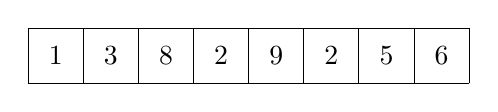
\begin{tikzpicture}[scale=0.7]
\draw (0,0) grid (8,1);
\node at (0.5,0.5) {$1$};
\node at (1.5,0.5) {$3$};
\node at (2.5,0.5) {$8$};
\node at (3.5,0.5) {$2$};
\node at (4.5,0.5) {$9$};
\node at (5.5,0.5) {$2$};
\node at (6.5,0.5) {$5$};
\node at (7.5,0.5) {$6$};
\end{tikzpicture}
\end{center}
排序后变为：
\begin{center}
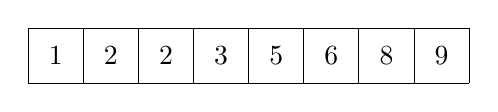
\begin{tikzpicture}[scale=0.7]
\draw (0,0) grid (8,1);
\node at (0.5,0.5) {$1$};
\node at (1.5,0.5) {$2$};
\node at (2.5,0.5) {$2$};
\node at (3.5,0.5) {$3$};
\node at (4.5,0.5) {$5$};
\node at (5.5,0.5) {$6$};
\node at (6.5,0.5) {$8$};
\node at (7.5,0.5) {$9$};
\end{tikzpicture}
\end{center}

\subsubsection{$O(n^2)$ 算法}

\index{bubble sort}

简单排序算法通常需要 $O(n^2)$ 时间。这类算法代码很短，一般由两个嵌套循环组成。著名的 $O(n^2)$ 排序算法是\key{冒泡排序}，其中元素会按数值大小在数组中逐渐“冒泡”。

冒泡排序进行 $n$ 轮。每一轮遍历数组元素，只要发现相邻两元素顺序不正确，就交换它们。实现如下：
\begin{lstlisting}
for (int i = 0; i < n; i++) {
    for (int j = 0; j < n-1; j++) {
        if (array[j] > array[j+1]) {
            swap(array[j],array[j+1]);
        }
    }
}
\end{lstlisting}

第一轮结束后，最大元素会到达正确位置；一般而言，经过 $k$ 轮后，最大的 $k$ 个元素都会位于正确位置。因此，经过 $n$ 轮后整个数组即已排序。

例如，对数组

\begin{center}
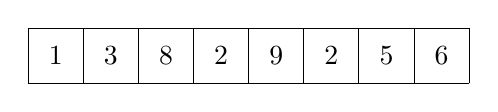
\begin{tikzpicture}[scale=0.7]
\draw (0,0) grid (8,1);

\node at (0.5,0.5) {$1$};
\node at (1.5,0.5) {$3$};
\node at (2.5,0.5) {$8$};
\node at (3.5,0.5) {$2$};
\node at (4.5,0.5) {$9$};
\node at (5.5,0.5) {$2$};
\node at (6.5,0.5) {$5$};
\node at (7.5,0.5) {$6$};
\end{tikzpicture}
\end{center}

\noindent
冒泡排序第一轮按如下过程交换元素：

\begin{center}
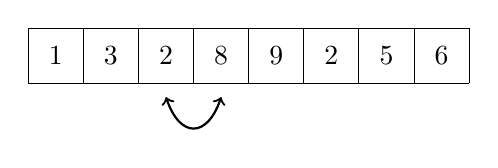
\begin{tikzpicture}[scale=0.7]
\draw (0,0) grid (8,1);
\node at (0.5,0.5) {$1$};
\node at (1.5,0.5) {$3$};
\node at (2.5,0.5) {$2$};
\node at (3.5,0.5) {$8$};
\node at (4.5,0.5) {$9$};
\node at (5.5,0.5) {$2$};
\node at (6.5,0.5) {$5$};
\node at (7.5,0.5) {$6$};

\draw[thick,<->] (3.5,-0.25) .. controls (3.25,-1.00) and (2.75,-1.00) .. (2.5,-0.25);
\end{tikzpicture}
\end{center}

\begin{center}
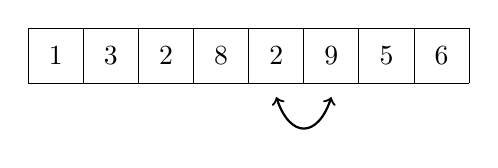
\begin{tikzpicture}[scale=0.7]
\draw (0,0) grid (8,1);
\node at (0.5,0.5) {$1$};
\node at (1.5,0.5) {$3$};
\node at (2.5,0.5) {$2$};
\node at (3.5,0.5) {$8$};
\node at (4.5,0.5) {$2$};
\node at (5.5,0.5) {$9$};
\node at (6.5,0.5) {$5$};
\node at (7.5,0.5) {$6$};

\draw[thick,<->] (5.5,-0.25) .. controls (5.25,-1.00) and (4.75,-1.00) .. (4.5,-0.25);
\end{tikzpicture}
\end{center}

\begin{center}
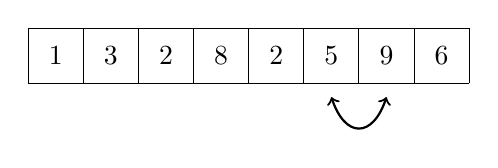
\begin{tikzpicture}[scale=0.7]
\draw (0,0) grid (8,1);
\node at (0.5,0.5) {$1$};
\node at (1.5,0.5) {$3$};
\node at (2.5,0.5) {$2$};
\node at (3.5,0.5) {$8$};
\node at (4.5,0.5) {$2$};
\node at (5.5,0.5) {$5$};
\node at (6.5,0.5) {$9$};
\node at (7.5,0.5) {$6$};

\draw[thick,<->] (6.5,-0.25) .. controls (6.25,-1.00) and (5.75,-1.00) .. (5.5,-0.25);
\end{tikzpicture}
\end{center}

\begin{center}
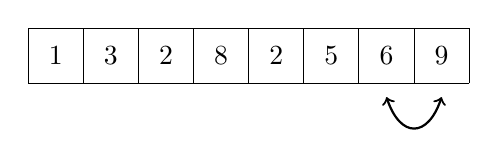
\begin{tikzpicture}[scale=0.7]
\draw (0,0) grid (8,1);
\node at (0.5,0.5) {$1$};
\node at (1.5,0.5) {$3$};
\node at (2.5,0.5) {$2$};
\node at (3.5,0.5) {$8$};
\node at (4.5,0.5) {$2$};
\node at (5.5,0.5) {$5$};
\node at (6.5,0.5) {$6$};
\node at (7.5,0.5) {$9$};

\draw[thick,<->] (7.5,-0.25) .. controls (7.25,-1.00) and (6.75,-1.00) .. (6.5,-0.25);
\end{tikzpicture}
\end{center}

\subsubsection{逆序对}

\index{inversion}

冒泡排序是一种始终交换数组中\emph{相邻}元素的排序算法。这类算法的时间复杂度\emph{必然}至少为 $O(n^2)$，因为最坏情况下需要 $O(n^2)$ 次交换才能把数组排好序。

分析排序算法时，一个实用概念是\key{逆序对}：一对数组元素 $(\texttt{array}[a],\texttt{array}[b])$，满足 $a<b$ 且 $\texttt{array}[a]>\texttt{array}[b]$，即两元素顺序错误。例如，数组
\begin{center}
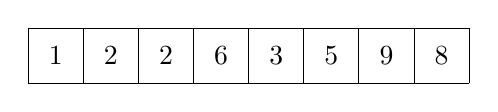
\begin{tikzpicture}[scale=0.7]
\draw (0,0) grid (8,1);
\node at (0.5,0.5) {$1$};
\node at (1.5,0.5) {$2$};
\node at (2.5,0.5) {$2$};
\node at (3.5,0.5) {$6$};
\node at (4.5,0.5) {$3$};
\node at (5.5,0.5) {$5$};
\node at (6.5,0.5) {$9$};
\node at (7.5,0.5) {$8$};
\end{tikzpicture}
\end{center}
有三个逆序对：$(6,3)$、$(6,5)$ 和 $(9,8)$。逆序对数量反映了数组排序所需的工作量。数组完全有序时没有逆序对；若元素完全逆序，逆序对数量达到最大：
\[1+2+\cdots+(n-1)=\frac{n(n-1)}{2} = O(n^2)\]

交换一对顺序错误的相邻元素，恰好消除一个逆序对。因此，若排序算法只能交换相邻元素，每次交换至多消除一个逆序对，其时间复杂度至少为 $O(n^2)$。

\subsubsection{$O(n \log n)$ 算法}

\index{merge sort}

不局限于交换相邻元素的算法，可以在 $O(n \log n)$ 时间内高效排序数组。其中一种是基于递归的\key{归并排序}\footnote{据文献 \cite{knu983}，归并排序由 J. von Neumann 于 1945 年发明。}。

归并排序按如下步骤排序子数组 \texttt{array}$[a \ldots b]$：

\begin{enumerate}
\item 若 $a=b$，子数组已经有序，无须操作。
\item 计算中间位置：$k=\lfloor (a+b)/2 \rfloor$。
\item 递归排序子数组 \texttt{array}$[a \ldots k]$。
\item 递归排序子数组 \texttt{array}$[k+1 \ldots b]$。
\item 将两个有序子数组 \texttt{array}$[a \ldots k]$ 与 \texttt{array}$[k+1 \ldots b]$ \emph{归并}成有序子数组 \texttt{array}$[a \ldots b]$。
\end{enumerate}

归并排序十分高效，因为每一步都会把子数组大小减半。递归共有 $O(\log n)$ 层，每层处理需要 $O(n)$ 时间。由于两个子数组已经有序，可以在线性时间内完成归并。

例如，考虑排序以下数组：
\begin{center}
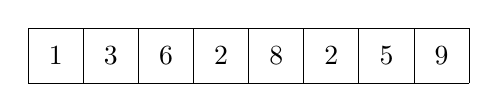
\begin{tikzpicture}[scale=0.7]
\draw (0,0) grid (8,1);
\node at (0.5,0.5) {$1$};
\node at (1.5,0.5) {$3$};
\node at (2.5,0.5) {$6$};
\node at (3.5,0.5) {$2$};
\node at (4.5,0.5) {$8$};
\node at (5.5,0.5) {$2$};
\node at (6.5,0.5) {$5$};
\node at (7.5,0.5) {$9$};
\end{tikzpicture}
\end{center}

数组先被分成两个子数组：
\begin{center}
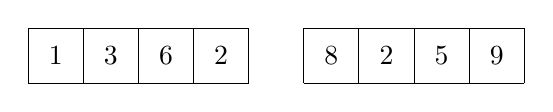
\begin{tikzpicture}[scale=0.7]
\draw (0,0) grid (4,1);
\draw (5,0) grid (9,1);

\node at (0.5,0.5) {$1$};
\node at (1.5,0.5) {$3$};
\node at (2.5,0.5) {$6$};
\node at (3.5,0.5) {$2$};

\node at (5.5,0.5) {$8$};
\node at (6.5,0.5) {$2$};
\node at (7.5,0.5) {$5$};
\node at (8.5,0.5) {$9$};
\end{tikzpicture}
\end{center}

随后递归排序两个子数组：
\begin{center}
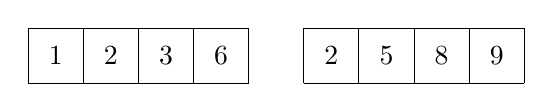
\begin{tikzpicture}[scale=0.7]
\draw (0,0) grid (4,1);
\draw (5,0) grid (9,1);

\node at (0.5,0.5) {$1$};
\node at (1.5,0.5) {$2$};
\node at (2.5,0.5) {$3$};
\node at (3.5,0.5) {$6$};

\node at (5.5,0.5) {$2$};
\node at (6.5,0.5) {$5$};
\node at (7.5,0.5) {$8$};
\node at (8.5,0.5) {$9$};
\end{tikzpicture}
\end{center}

最后，算法归并两个有序子数组，得到最终的有序数组：
\begin{center}
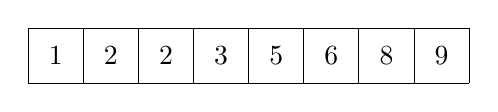
\begin{tikzpicture}[scale=0.7]
\draw (0,0) grid (8,1);
\node at (0.5,0.5) {$1$};
\node at (1.5,0.5) {$2$};
\node at (2.5,0.5) {$2$};
\node at (3.5,0.5) {$3$};
\node at (4.5,0.5) {$5$};
\node at (5.5,0.5) {$6$};
\node at (6.5,0.5) {$8$};
\node at (7.5,0.5) {$9$};
\end{tikzpicture}
\end{center}

\subsubsection{排序下界}

能否比 $O(n \log n)$ 更快地排序数组？若只考虑基于元素比较的排序算法，答案是\emph{不能}。

可以把排序看作一个过程：每比较两个元素一次，就获得更多关于数组内容的信息。该过程形成如下决策树，由此可以证明时间复杂度下界：

\begin{center}
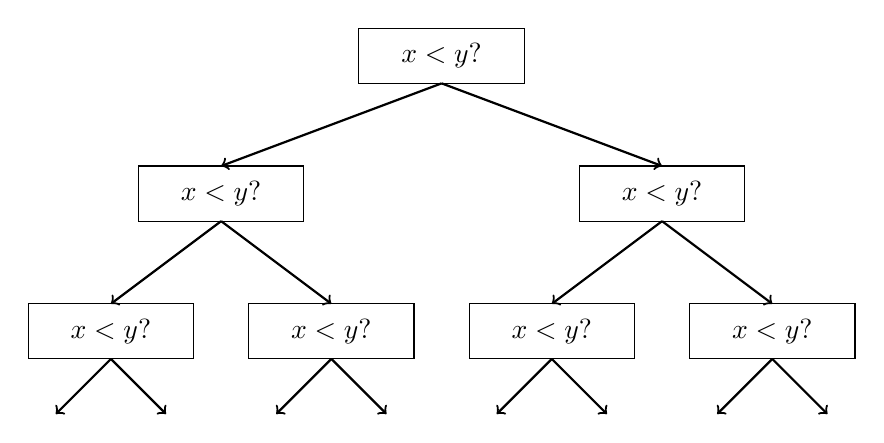
\begin{tikzpicture}[scale=0.7]
\draw (0,0) rectangle (3,1);
\node at (1.5,0.5) {$x < y?$};

\draw[thick,->] (1.5,0) -- (-2.5,-1.5);
\draw[thick,->] (1.5,0) -- (5.5,-1.5);

\draw (-4,-2.5) rectangle (-1,-1.5);
\draw (4,-2.5) rectangle (7,-1.5);
\node at (-2.5,-2) {$x < y?$};
\node at (5.5,-2) {$x < y?$};

\draw[thick,->] (-2.5,-2.5) -- (-4.5,-4);
\draw[thick,->] (-2.5,-2.5) -- (-0.5,-4);
\draw[thick,->] (5.5,-2.5) -- (3.5,-4);
\draw[thick,->] (5.5,-2.5) -- (7.5,-4);

\draw (-6,-5) rectangle (-3,-4);
\draw (-2,-5) rectangle (1,-4);
\draw (2,-5) rectangle (5,-4);
\draw (6,-5) rectangle (9,-4);
\node at (-4.5,-4.5) {$x < y?$};
\node at (-0.5,-4.5) {$x < y?$};
\node at (3.5,-4.5) {$x < y?$};
\node at (7.5,-4.5) {$x < y?$};

\draw[thick,->] (-4.5,-5) -- (-5.5,-6);
\draw[thick,->] (-4.5,-5) -- (-3.5,-6);
\draw[thick,->] (-0.5,-5) -- (0.5,-6);
\draw[thick,->] (-0.5,-5) -- (-1.5,-6);
\draw[thick,->] (3.5,-5) -- (2.5,-6);
\draw[thick,->] (3.5,-5) -- (4.5,-6);
\draw[thick,->] (7.5,-5) -- (6.5,-6);
\draw[thick,->] (7.5,-5) -- (8.5,-6);
\end{tikzpicture}
\end{center}

其中“$x<y?$”表示比较元素 $x$ 与 $y$。若 $x<y$，过程向左继续，否则向右继续。过程的结果对应数组所有可能的排列，共有 $n!$ 种。因此，树高至少为
\[ \log_2(n!) = \log_2(1)+\log_2(2)+\cdots+\log_2(n).\]
取和式最后 $n/2$ 项，并把每项改为 $\log_2(n/2)$，可得到下界估计
\[ \log_2(n!) \ge (n/2) \cdot \log_2(n/2),\]
因此，决策树高度以及排序算法最坏情况下所需的最少步骤数，至少为 $n \log n$ 量级。

\subsubsection{计数排序}

\index{counting sort}

对于不比较数组元素、而利用其他信息的算法，$n \log n$ 下界并不成立。\key{计数排序}就是一例：若数组每个元素都是 $0 \ldots c$ 范围内的整数，且 $c=O(n)$，它可以在 $O(n)$ 时间内完成排序。

算法创建一个\emph{计数}数组，其下标对应原数组中的元素。遍历原数组，统计每个元素的出现次数。
\newpage

例如，数组
\begin{center}
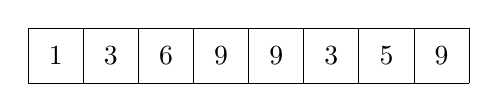
\begin{tikzpicture}[scale=0.7]
\draw (0,0) grid (8,1);
\node at (0.5,0.5) {$1$};
\node at (1.5,0.5) {$3$};
\node at (2.5,0.5) {$6$};
\node at (3.5,0.5) {$9$};
\node at (4.5,0.5) {$9$};
\node at (5.5,0.5) {$3$};
\node at (6.5,0.5) {$5$};
\node at (7.5,0.5) {$9$};
\end{tikzpicture}
\end{center}
对应如下计数数组：
\begin{center}
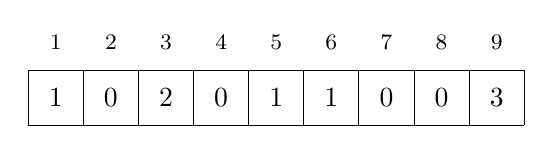
\begin{tikzpicture}[scale=0.7]
\draw (0,0) grid (9,1);
\node at (0.5,0.5) {$1$};
\node at (1.5,0.5) {$0$};
\node at (2.5,0.5) {$2$};
\node at (3.5,0.5) {$0$};
\node at (4.5,0.5) {$1$};
\node at (5.5,0.5) {$1$};
\node at (6.5,0.5) {$0$};
\node at (7.5,0.5) {$0$};
\node at (8.5,0.5) {$3$};

\footnotesize

\node at (0.5,1.5) {$1$};
\node at (1.5,1.5) {$2$};
\node at (2.5,1.5) {$3$};
\node at (3.5,1.5) {$4$};
\node at (4.5,1.5) {$5$};
\node at (5.5,1.5) {$6$};
\node at (6.5,1.5) {$7$};
\node at (7.5,1.5) {$8$};
\node at (8.5,1.5) {$9$};
\end{tikzpicture}
\end{center}

例如，计数数组位置 3 的值为 2，因为元素 3 在原数组中出现了两次。

构造计数数组需要 $O(n)$ 时间。随后，可根据每个元素的出现次数，在 $O(n)$ 时间内生成有序数组。因此，计数排序的总时间复杂度为 $O(n)$。

计数排序非常高效，但只有当常数 $c$ 足够小、数组元素能够作为计数数组下标时才能使用。

\section{C++ 中的排序}

\index{sort@\texttt{sort}}

竞赛中几乎不应自行实现排序算法，因为编程语言已经提供了优秀实现。例如，C++ 标准库中的 \texttt{sort} 函数可轻松用于排序数组及其他数据结构。

使用库函数有很多好处。首先，无须自行实现，能够节省时间；其次，库实现可以确信是正确且高效的，自写排序函数通常不会更好。

本节介绍 C++ 的 \texttt{sort} 函数。下面的代码将向量按递增顺序排序：
\begin{lstlisting}
vector<int> v = {4,2,5,3,5,8,3};
sort(v.begin(),v.end());
\end{lstlisting}
排序后，向量内容为 $[2,3,3,4,5,5,8]$。默认排序顺序为递增，也可按如下方式改为递减：
\begin{lstlisting}
sort(v.rbegin(),v.rend());
\end{lstlisting}
普通数组可按如下方式排序：
\begin{lstlisting}
int n = 7; // array size
int a[] = {4,2,5,3,5,8,3};
sort(a,a+n);
\end{lstlisting}
\newpage
下面的代码对字符串 \texttt{s} 排序：
\begin{lstlisting}
string s = "monkey";
sort(s.begin(), s.end());
\end{lstlisting}
对字符串排序是指排列其中的字符。例如，字符串 ``monkey'' 会变为 ``ekmnoy''。

\subsubsection{比较运算符}

\index{comparison operator}

\texttt{sort} 要求待排序元素的数据类型定义了\key{比较运算符}。排序过程中，每当需要确定两个元素的先后顺序时，就会使用该运算符。

大多数 C++ 数据类型都内置了比较运算符，可以自动排序。例如，数字按数值排序，字符串按字典序排序。

\index{pair@\texttt{pair}}

二元组（\texttt{pair}）首先按第一元素（\texttt{first}）排序；若第一元素相等，再按第二元素（\texttt{second}）排序：
\begin{lstlisting}
vector<pair<int,int>> v;
v.push_back({1,5});
v.push_back({2,3});
v.push_back({1,2});
sort(v.begin(), v.end());
\end{lstlisting}
此后二元组顺序为 $(1,2)$、$(1,5)$、$(2,3)$。

\index{tuple@\texttt{tuple}}

类似地，元组（\texttt{tuple}）依次按第一元素、第二元素等排序\footnote{注意，在某些旧编译器中，必须用函数 \texttt{make\_tuple} 而非花括号创建元组（例如用 \texttt{make\_tuple(2,1,4)} 代替 \texttt{\{2,1,4\}}）。}：
\begin{lstlisting}
vector<tuple<int,int,int>> v;
v.push_back({2,1,4});
v.push_back({1,5,3});
v.push_back({2,1,3});
sort(v.begin(), v.end());
\end{lstlisting}
此后元组顺序为 $(1,5,3)$、$(2,1,3)$、$(2,1,4)$。

\subsubsection{自定义结构体}

自定义结构体不会自动拥有比较运算符。应在结构体内部定义函数 \texttt{operator<}，其参数为同类型的另一个元素。若当前元素小于参数，运算符应返回 \texttt{true}，否则返回 \texttt{false}。

例如，下面的结构体 \texttt{P} 包含一个点的 x、y 坐标。比较运算符使各点首先按 x 坐标排序，其次按 y 坐标排序。

\begin{lstlisting}
struct P {
    int x, y;
    bool operator<(const P &p) {
        if (x != p.x) return x < p.x;
        else return y < p.y;
    }
};
\end{lstlisting}

\subsubsection{比较函数}

\index{comparison function}

也可以把外部\key{比较函数}作为回调函数传给 \texttt{sort}。例如，下面的比较函数 \texttt{comp} 首先按长度、其次按字典序排列字符串：

\begin{lstlisting}
bool comp(string a, string b) {
    if (a.size() != b.size()) return a.size() < b.size();
    return a < b;
}
\end{lstlisting}
此时可按如下方式排序字符串向量：
\begin{lstlisting}
sort(v.begin(), v.end(), comp);
\end{lstlisting}

\section{二分查找}

\index{binary search}

在数组中查找元素的一般方法是用 \texttt{for} 循环遍历数组。例如，下面的代码查找元素 $x$：

\begin{lstlisting}
for (int i = 0; i < n; i++) {
    if (array[i] == x) {
        // x found at index i
    }
}
\end{lstlisting}

该方法时间复杂度为 $O(n)$，因为最坏情况下必须检查所有元素。若元素顺序任意，这也是最优方法，因为没有额外信息能指示应在数组何处寻找 $x$。

若数组\emph{有序}，情况就不同了。元素顺序可以指导搜索，使查找大幅加速。下面的\key{二分查找}能在 $O(\log n)$ 时间内高效查找有序数组中的元素。

\subsubsection{方法一}

二分查找的常见实现类似于在词典中查找单词。查找过程维护数组中的一个活动区间，初始包含全部元素；随后执行若干步，每一步都把区间大小减半。

每一步检查活动区间的中间元素。若它就是目标元素，搜索结束；否则根据中间元素的值，继续搜索左半或右半区间。

上述思想可实现如下：
\begin{lstlisting}
int a = 0, b = n-1;
while (a <= b) {
    int k = (a+b)/2;
    if (array[k] == x) {
        // x found at index k
    }
    if (array[k] > x) b = k-1;
    else a = k+1;
}
\end{lstlisting}

该实现中的活动区间为 $a \ldots b$，初始为 $0 \ldots n-1$。算法每一步都把区间大小减半，所以时间复杂度为 $O(\log n)$。

\subsubsection{方法二}

另一种二分查找实现基于高效遍历数组元素。其思想是进行跳跃，并在接近目标元素时逐渐缩短步长。

搜索从左向右进行，初始跳跃长度为 $n/2$。每一步把跳跃长度减半，依次变为 $n/4$、$n/8$、$n/16$ 等，直至 1。跳跃结束后，要么已经找到目标元素，要么确定它不在数组中。

实现如下：
\begin{lstlisting}
int k = 0;
for (int b = n/2; b >= 1; b /= 2) {
    while (k+b < n && array[k+b] <= x) k += b;
}
if (array[k] == x) {
    // x found at index k
}
\end{lstlisting}

搜索过程中，变量 $b$ 存储当前跳跃长度。算法时间复杂度为 $O(\log n)$，因为对每种跳跃长度，\texttt{while} 循环中的代码至多执行两次。

\subsubsection{C++ 函数}

C++ 标准库提供以下基于二分查找、在对数时间内运行的函数：

\begin{itemize}
\item \texttt{lower\_bound} 返回指向第一个值不小于 $x$ 的数组元素的指针。
\item \texttt{upper\_bound} 返回指向第一个值大于 $x$ 的数组元素的指针。
\item \texttt{equal\_range} 同时返回上述两个指针。
\end{itemize}

这些函数假设数组已经有序。若不存在满足条件的元素，指针会指向数组末尾元素之后的位置。例如，下面的代码判断数组是否包含值为 $x$ 的元素：

\begin{lstlisting}
auto k = lower_bound(array,array+n,x)-array;
if (k < n && array[k] == x) {
    // x found at index k
}
\end{lstlisting}

下面的代码统计值为 $x$ 的元素数量：

\begin{lstlisting}
auto a = lower_bound(array, array+n, x);
auto b = upper_bound(array, array+n, x);
cout << b-a << "\n";
\end{lstlisting}

使用 \texttt{equal\_range} 可以缩短代码：

\begin{lstlisting}
auto r = equal_range(array, array+n, x);
cout << r.second-r.first << "\n";
\end{lstlisting}

\subsubsection{寻找最小解}

二分查找的一项重要用途是找到某个\emph{函数}值发生变化的位置。假设要找出问题的最小可行解 $k$。给定函数 $\texttt{ok}(x)$：若 $x$ 是可行解则返回 \texttt{true}，否则返回 \texttt{false}。还已知当 $x<k$ 时函数为 \texttt{false}，当 $x \ge k$ 时为 \texttt{true}。情况如下：

\begin{center}
\begin{tabular}{r|rrrrrrrr}
$x$ & 0 & 1 & $\cdots$ & $k-1$ & $k$ & $k+1$ & $\cdots$ \\
\hline
$\texttt{ok}(x)$ & \texttt{false} & \texttt{false}
& $\cdots$ & \texttt{false} & \texttt{true} & \texttt{true} & $\cdots$ \\
\end{tabular}
\end{center}

\noindent
可以用二分查找求出 $k$：

\begin{lstlisting}
int x = -1;
for (int b = z; b >= 1; b /= 2) {
    while (!ok(x+b)) x += b;
}
int k = x+1;
\end{lstlisting}

搜索会找到满足 $\texttt{ok}(x)$ 为 \texttt{false} 的最大 $x$。因此，下一个值 $k=x+1$ 就是使 $\texttt{ok}(k)$ 为 \texttt{true} 的最小值。初始跳跃长度 $z$ 必须足够大，例如预先知道 $\texttt{ok}(z)$ 为 \texttt{true} 的某个值。

算法调用函数 \texttt{ok} 共 $O(\log z)$ 次，因此总时间复杂度取决于 \texttt{ok}。例如，若该函数运行时间为 $O(n)$，则总复杂度为 $O(n \log z)$。

\subsubsection{寻找最大值}

二分查找还可用于求一个先增后减函数的最大值。目标是找出位置 $k$，使得

\begin{itemize}
\item
$f(x)<f(x+1)$ when $x<k$, and
\item
$f(x)>f(x+1)$ when $x \ge k$.
\end{itemize}

方法是用二分查找找到满足 $f(x)<f(x+1)$ 的最大 $x$。由于此时 $f(x+1)>f(x+2)$，所以 $k=x+1$。实现如下：

\begin{lstlisting}
int x = -1;
for (int b = z; b >= 1; b /= 2) {
    while (f(x+b) < f(x+b+1)) x += b;
}
int k = x+1;
\end{lstlisting}

注意，与普通二分查找不同，这里不允许函数的相邻值相等，否则无法判断搜索应向哪一侧继续。
